We consider the settling aggregate in a constant density fluid. To describe the incompressible fluid flow, it is general to consider the Navier-Stokes equations,
\begin{align}
\nabla \cdot \vec{u}(\vec{y}) = 0 
\\
\rho \frac{D\vec{u}(\vec{y})}{Dt}
 =\mu \nabla^2 \vec{u}(\vec{y}) - \nabla P(\vec{y}) + \rho  \vec{g} ,
\label{eq_momentum_NS}
\end{align}
where $\vec{u}, \ \mu, \ P, \ \rho$ are fluid velocity, viscosity, pressure, and constant density, respectively. Also, the gravitaty vector is $\vec{g} = - g\hat{k} \approx (0,0,-9.8$m/$s^2)$ and $\vec{y} \in \mathbb{R}^3$ represents an arbitrary point in the fluid domain. 
Note that $D$ is the material derivative, defined as
\begin{equation}
\frac{D}{Dt} = \frac{\partial}{\partial t} + \vec{u}\cdot \nabla.
\end{equation}
Considering the settling speed and size of a typical aggregate, we may linearize the momentum equation (\ref{eq_momentum_NS}) in the limit of zero Reynolds number. We begin with introducing the Reynolds number we obtain in the following section. 
\section{Governing equations}
{\color{blue} MAKE SURE THE NUMBERS ARE CONSISTENT WITH THE CODE.}
The marine aggregates are typically small and porous with a maximum radius, $R_a$, of about $ 500 \mu \text{m}$.
%porosities on the order of 99$\%$ of the aggregates. 
With all the values given, we obtain a maximum Reynolds number of,
\begin{equation*}
    \text{Re} = \frac{\rho U_s R_a}{\mu} 
	% \approx 5 \times 10^{-2} 
	\ll 1.
\end{equation*}
Note that $U_s$ is a reference Stokes settling speed of an aggregate, defined by, 
\begin{equation}
    U_s =  \frac{gR_a^2}{\mu} (\rho_a-\rho) \approx 3 \times 10^{-4} ({\text{m/s}}),
	\label{eq_U_s}
\end{equation}
where $\rho_a$ is the aggregate mass density. Since the Reynolds number is fairly small, we can use the Stokes equations, ignoring the inertial effects.
 We thus consider the Stokes equations to describe the fluid flow around the settling aggregates,
 \begin{align}
	\nabla \cdot \vec{u} (\vec{y}) = 0  \label{eq_conti2}
	\\
	\mu \nabla^2 \vec{u} (\vec{y})   - \nabla P(\vec{y}) \ + \rho  \vec{g} = 0
	\label{eq_stokes2}
\end{align}
where $\mu$ and $\rho$ are the viscosity and density of the fluid, respectively. The solutions of the equations are the fluid velocity, $\vec{u}$, and pressure, $P$. For the parameters, we assume typical seawater quantities:  $\rho \approx 1020 \text{kg/m}^3$ and $\mu = 1.5 \times 10^{-3}\text{kg}/\text{ms}$. Also, $g \approx 9.8 \text{m/s}^2$ is the gravitational acceleration.
%
%
%
%===SECTION 2.2=========================================
\section{Boundary integral equation (BIE) formulations} 
$\ \ \ \ $ 
We use a BIE formulation to represent the solution of the Stokes equations. One advantage of this form is the reduction of dimension; we solve a three-dimensional flow with a two-dimensional integral equation. 
In order to use a BIE, we assume that the velocity vanishes at infinity and the aggregate is solid. Although marine aggregates are porous, the solid boundary condition is reasonable to apply due to their is low permeability. This condition prevents a flow through the aggregate, acting like a solid particle. For this reason, any flow inside of the aggregate is out of our interest.  
\par
The representation formula for the velocity solution, $\vec{u}$, to the Stokes equations at any point $\vec{y} \in \mathbb{R}^3$ that is outside of a solid object boundary, $S(\vec{x})$, is
% around a solid object is expressed, using the stress vector, $\vec{f}$, 
\begin{equation}
   \vec{u}(\vec{y}) =
	- \frac{1}{8 \pi \mu} \int_S  \vec{f}(\vec{x}) \cdot \bar{\bar{G}}(\vec{x},\vec{y}) \ \text{d}S(\vec{x}) 
+ \frac{1}{8 \pi} \int_S
\vec{u}(\vec{x}) \cdot  \bar{\bar{T}}(\vec{x},\vec{y})  
\cdot \hat{n} ( \vec{x})
\ \text{d}S(\vec{x}),
\label{eq_BIE}
\end{equation}
where  $\vec{f}$ is the stress vector \cite{pozrikidis_boundary_1992}.
The first integral distribution on the right-hand side of equation (\ref{eq_BIE}) is called the \textit{single-layer potential} and the second one is called the \textit{double-layer potential}. 
To compute the velocity at a point on the surface $S$, i.e., $ \vec{x}_s \in S$, we have 
\begin{equation}
   \vec{u}(\vec{x}_s) = - \frac{1}{4 \pi \mu} \int_S  \vec{f}(\vec{x}) \cdot \bar{\bar{G}}(\vec{x},\vec{x}_s) \ \text{d}S(\vec{x}) 
+ \frac{1}{4 \pi} 
\int_S
\vec{u}(\vec{x}) \cdot  \bar{\bar{T}}(\vec{x},\vec{x}_s)  
\cdot \hat{n} ( \vec{x})
\ \text{d}S(\vec{x}).
\label{eq_BIE_onS}
\end{equation}
The second order tensors in equation (\ref{eq_BIE}) are the Green's function,  $\bar{\bar{G}}(\vec{x},\vec{y})$,
\begin{align}
  \bar{\bar{G}}(\vec{x},\vec{y}) =   
  \frac{\bar{\bar{I}}}{||\vec{x}-\vec{y}||} + \frac{(\vec{x}-\vec{y})(\vec{x}-\vec{y})}{||\vec{x}-\vec{y}||^3},
  \label{eq_stokeslet}
  \end{align}
  and the stress tensor, $\bar{\bar{T}}(\vec{x},\vec{y})$ , associated with the Green's function of the Stokes equations,
  %
  \begin{align}
  \bar{\bar{T}}(\vec{x},\vec{y}) = 
  -6\frac{(\vec{x}-\vec{y})(\vec{x}-\vec{y}) (\vec{x}-\vec{y})}{||\vec{x}-\vec{y}||^5},
  \label{eq_stresslet}
  \end{align}
where $\| \cdot \|$ is the $L^2$ norm. 
Note that $ \bar{\bar{G}}(\vec{x},\vec{y})$ and $ \bar{\bar{T}}(\vec{x},\vec{y}) $ are called  the {\textit{Stokeslet}} and {\textit{Stresslet}}, respectively.
\par
From the representation formula (\ref{eq_BIE}), we are able to simplify by eliminating one of layer potentials. 
In the rest of this section, we derive the equations with either the single- or double-layer potential only. 
%--------------------------------------------------------
\subsection{Single-layer potential}
$\ \ \ \ \ $ 
We first derive the velocity with the single-layer potential alone.
The solid boundary allows us to express its velocity as 
\begin{equation}
	\vec{u}_s \left( \vec{x} \right) 
	= \vec{U}_a + \vec{\Omega} \times \vec{x}  ,
	\label{eq_solid_vel}
\end{equation}
where $\vec{U}_a$ and $\vec{\Omega}$ are constant translational and angular velocities, respectively. 
Substituting the solid object velocity, equation (\ref{eq_solid_vel}), into the double-layer potential in equation (\ref{eq_BIE}) shows that 
\begin{align}
	\int_S
	\left( \vec{U}_a + \vec{\Omega} \times \vec{x} \right)
	 \cdot  \bar{\bar{T}}(\vec{x},\vec{y})  
	\cdot \hat{n} ( \vec{x})
	\ \text{d}S(\vec{x})
    \nonumber \\
	= 
	\int_S
	\vec{U}_a
	 \cdot  \bar{\bar{T}}(\vec{x},\vec{y})  
	\cdot \hat{n} ( \vec{x})
	\ \text{d}S(\vec{x})
     + 	
	\int_S
	\left(  \vec{\Omega} \times \vec{x} \right)
	 \cdot  \bar{\bar{T}}(\vec{x},\vec{y})  
	\cdot \hat{n} ( \vec{x})
	\ \text{d}S(\vec{x})
	\label{eq_solid_motion_dlp}
\end{align}
% We consider two flows, $\vec{U}_a$ and $\vec{\Omega}$, separately. 
The first integral of the right-hand side of equation (\ref{eq_solid_motion_dlp}) can be re-written as 
\begin{equation}
	\vec{U}_a \cdot
	\int_S
	  \bar{\bar{T}}(\vec{x},\vec{y})  
	\cdot \hat{n} ( \vec{x})
	\ \text{d}S(\vec{x}),
	\label{eq_solid_motion_dlp_Ua}
\end{equation}
since the translational velocity, $\vec{U}_a$, is constant. 
For the flow around (outside) and on the solid object, Pozrikidis provides an useful identity \cite{pozrikidis_boundary_1992} (page 21, equation (2.1.12))
\begin{align}
	\int_S  \bar{\bar{T}}(\vec{x},\vec{y}) \cdot \hat{n} ( \vec{x})
	\ \text{d}S(\vec{x})
	=
	 \begin{cases}
	 \bar{\bar{0}} & \text{ if } \vec{y} \in \mathbb{R}^3  \setminus  \left( S \cup {\text{inside of aggregate}}\right) 	\\ 
	 - 4\pi \bar{\bar{I}} & \text{ if } \vec{y} \in S 
	 \end{cases}.
	\label{eq_dlp_identity1}
\end{align}
Then, including the velocity $\vec{U}_a$, we get
\begin{align}
	\vec{U}_a \cdot
	\int_S  \bar{\bar{T}}(\vec{x},\vec{y}) \cdot \hat{n} ( \vec{x})
	\ \text{d}S(\vec{x})
	=
	 \begin{cases}
	 \vec{0}& \text{ if } \vec{y} \in \mathbb{R}^3  \setminus \left( S \cup {\text{inside of aggregate}}\right) 	\\ 
	 - 4\pi \vec{U}_a  & \text{ if } \vec{y} \in S 
	 \end{cases}.
	\label{eq_dlp_Ua}
\end{align}
% Applying these values to the representation formulae, equation(\ref{eq_BIE}) and (\ref{eq_BIE_onS}), allows us to remove the double-layer potential.
\par 
The second integral in equation (\ref{eq_solid_motion_dlp}) can be evaluated with the following identity, from \cite{pozrikidis_boundary_1992},
using Einstein (summation) notation, 
\begin{align}
	\varepsilon_{i \ell m}
	\int_S x_{\ell} \ T_{mjk}(\vec{x},\vec{y})  \ n_{k} ( \vec{x})
	\ \text{d}S(\vec{x})
	 = 
	 \begin{cases}
	  \vec{0}
	  & \text{ if } \vec{y} \in \mathbb{R}^3  \setminus  	\left( S \cup {\text{inside of aggregate}}\right) \\ 
	 - 4\pi \ \varepsilon_{i \ell j} \ x_{\ell}
	 & \text{ if } \vec{y} \in S 
	 \end{cases},
	\label{eq_dlp_identity2}
\end{align}
where $\varepsilon_{i \ell m}$ is the Levi-Civita permutation symbol.  
Multiplying both sides by the angular velocity, $\Omega$, in equation (\ref{eq_dlp_identity2}), we get 
\begin{align}
	&
	\int_S
	\left( \vec{\Omega} \times \vec{x} \right)
	 \cdot  \bar{\bar{T}}(\vec{x},\vec{x}_s)  
	\cdot \hat{n} ( \vec{x})
	\ \text{d}S(\vec{x})
	 = 
	\int_S 
	\left(  \varepsilon_{i \ell m} \ \Omega_{i} x_{\ell} \right) \ 	T_{mjk}(\vec{x},\vec{y})  \ n_{k} ( \vec{x})
	\ \text{d}S(\vec{x})
	\nonumber \\
	\nonumber \\
 	& = 
 	\begin{cases}
 	  \vec{0}
 	 &  \\ 
 	- 4\pi \ \varepsilon_{i \ell j}\  \Omega_{i} \ x^0_{\ell}
 	& 
 	\end{cases}
	= \begin{cases}
 	  \vec{0}
 	 & \text{ if } \vec{y} \in \mathbb{R}^3  \setminus  
	 \left( S \cup {\text{inside of aggregate}}\right)
	  \\ 
 	- 4\pi \left(  \Omega \times \vec{y} \right)
 	& \text{ if } \vec{y} \in S.
 	\end{cases}
	\label{eq_dlp_Omega}
\end{align}
We now combine two equations, (\ref{eq_dlp_Ua}) and (\ref{eq_dlp_Omega}),
\begin{equation}
	\int_S \vec{u} ( \vec{x}) \cdot \bar{\bar{T}}(\vec{x},\vec{y}) \cdot \hat{n} ( \vec{x})
	\ \text{d}S(\vec{x})
	 = 
	 \begin{cases}
	  \vec{0}& \text{ if } \vec{y} \in \mathbb{R}^3  \setminus \left( S \cup {\text{inside of aggregate}}\right)
	  \\ 
	 - 4\pi \vec{u}(\vec{y}) & \text{ if } \vec{y} \in S 
	 \end{cases}.
	\label{eq_dlp_val_out}
\end{equation}
When the point $\vec{y}$ is strictly outside of the aggregate surface, $S$,
 \begin{equation}
    \vec{u}(\vec{y}) = - \frac{1}{8 \pi \mu} \int_S  \vec{f}(\vec{x}) \cdot \bar{\bar{G}}(\vec{x},\vec{y}) \ \text{d}S(\vec{x}) ,
 \label{eq_slp}
 \end{equation}
 only the single-layer potential term.
For evaluation points on the surface $S$, 
$\vec{y} = \vec{x}_s \in S$, 
since the double-layer potential is $- 4 \pi \vec{u}(\vec{x}_s)$, when we substitue into equation (\ref{eq_BIE_onS}), 
we obtain exactly the same equation (\ref{eq_slp}). This implies that the single-layer potential formula is continuous across the boundary surface $S$.
To analyze the force and torque, we use the stress $\vec{f}$ in equation (\ref{eq_slp}) as
\begin{equation}
 \vec{F}_o
  = \int_S \vec{f}(\vec{x}) \  \text{d}S(\vec{x})
 % = \int_S  \vec{\psi}( \vec{x}) \ \text{d}S(\vec{x}),
 \label{eq_total_Force_slp}
 \end{equation} 
 and
 \begin{equation}
 \vec{Q}_o  
 = \int_S (\vec{x} - \vec{x}_{cm}) \times \vec{f}(\vec{x})  \ \text{d}S (\vec{x})
 % =  \int_S  (\vec{x} - \vec{x}_{cm}) \times \vec{\psi}(\vec{x}) \ \text{d}S(\vec{x}).
 \label{eq_total_Torque_slp},
 \end{equation}
 where $\vec{F}_o$ and $\vec{Q}_o$ represent the total force and torque, respectively, acting on the aggregate surface $S$.
%
% Note that the single-layer potential is continuous across the surface boundary as long as the surface is smooth in general. The following theorem is cited from \cite{kress_linear_2014}.
% \begin{thm}
% 	Let $S$ be of class $C^2$ and $f \in C(S)$. Then the single-layer potential $u$ with density $f$ is continuous throughout $\mathbb{R}^m$. On the boundary $S$, we have
% 	\begin{equation*}
% 		u(x) = \int_S f(y) G(x,y) \ \text{d}S(y), \ \ \ x \in S,
% 	\end{equation*}
% 	where the integral exists as an improper integral.
% 	\label{eq_thm1}
% \end{thm}
% Although our aggregate model is not smooth overall with edges and corners, the idea of theorem (\ref{eq_thm1}) is valid for our approximation since we only use the boundary integral equations on the center of each discretized square face. We discuss details in the next chapter.

\subsection{Double-layer potential}
$\ \ \ \ \ $ 
In this section, we derive a velocity formulation, $\vec{u}$, using the double-layer potential. We shall consider a complimentary flow $\vec{u}_c$ 
% (not to be confused with the derivative prime notation) 
for the points inside of the aggregate surface boundary $S$, having the same force on the boundary as $\vec{u}$. Before we proceed, we need to prove the existence of the complimentary flow.
The new flow $\vec{u}_c$ can be found when the velocity $\vec{u}(\vec{x})$ at the boundary satisfies
\begin{equation}
 	\int_S \vec{u}(\vec{x}) \cdot \hat{n} \ \text{d}S(\vec{x})=0. 
	\label{eq_dlp_constraint}
\end{equation}
This condition is taken from \cite{pozrikidis_boundary_1992}.
This can be fulfilled with our problem due to the continuity equation, $\nabla \cdot \vec{u}= 0$ and divergence theorem.
% By the divergence theorem, equation \ref{eq_constraint} is equivalent to
\begin{figure}[h]
	\begin{center}
		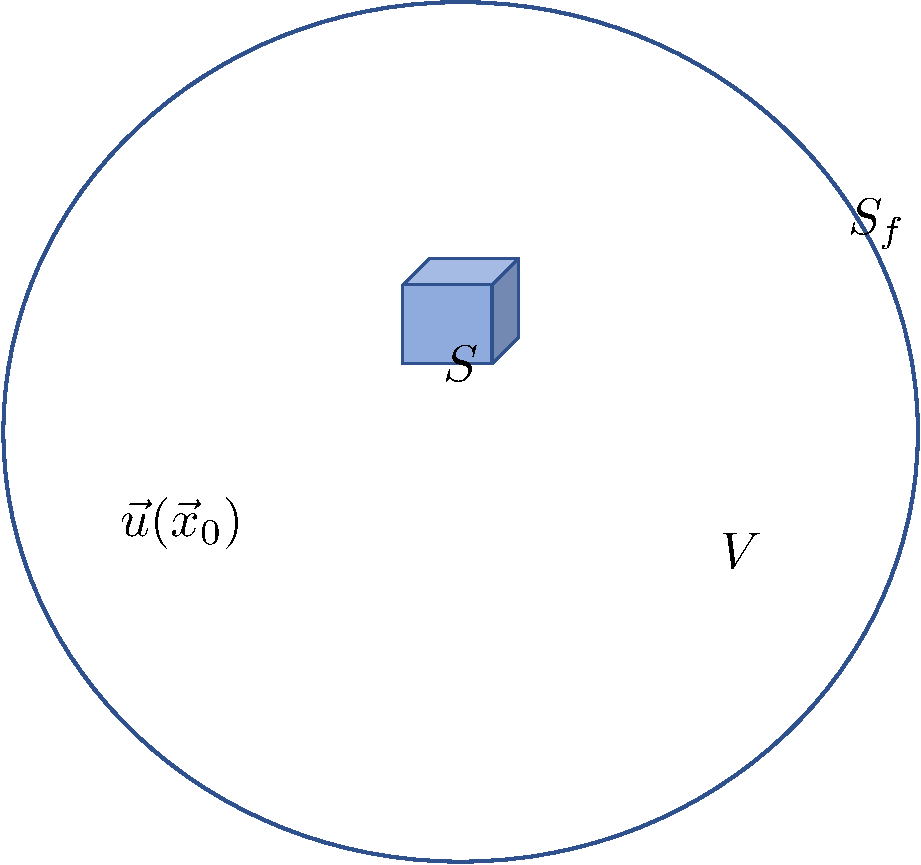
\includegraphics[scale=0.4]{./figures/fig_dlp_volume}
		\vspace{0.5cm}
	\caption{Schematic of the control volume and its surface.}
	\label{fig_dlp_volume}
\end{center}
\end{figure}
We first see that
\begin{equation}
 	\int_V  \nabla \cdot \vec{u}(\vec{x}) \ \text{d}V (\vec{x}) 
		=0. 
	\label{eq_constraint_v}
\end{equation}
By divergence theorem, we have
\begin{equation}
	\int_V  \nabla \cdot \vec{u}(\vec{x}) \ \text{d}V (\vec{x})   = 
\int_{S } \vec{u}(\vec{x}) \cdot \hat{n} \ \text{d}S(\vec{x})
+ \int_{S_f} \vec{u}(\vec{x}) \cdot \hat{n} \ \text{d}S(\vec{x})=0,
\label{eq_div}
\end{equation}
where $S_f$ is the surface of the control volume of the fluid surrounding the solid particle. 
We consider the surface $S_f$ as a large sphere with a radius $r_f$. Then the velocity $\vec{u}$ on $S_f$ approaches to zero with the order of $\mathcal{O}(1/r_f)$ and its associated stress tensor decays with the rate $\mathcal{O} (1/r_f^2)$. Once the surface integral on $S_f$ in equation (\ref{eq_div}) becomes zero, it implies that
\[
\int_{S} \vec{u}(\vec{x}) \cdot \hat{n} \ \text{d}S(\vec{x}) = 0.
\]
 It also means that the net force on the surface $S$ is zero. 

More specifically, the velocity $\vec{u}$  has the representation form, equation (\ref{eq_BIE}) and the complimentary flow $\vec{u}_c$ has the same stress, $\vec{f}$, on the boundary as $\vec{u}$. By the Lorentz reciprocal identity, any two flows having the same force on the boundary satisfy
% pozrikidis equation (2.3.26)
\begin{equation}
	\int_{S}  \vec{f}(\vec{x}) \cdot \bar{\bar{G}}(\vec{x},\vec{x}_o) \ \text{d}S(\vec{x})  
	- \mu \int_S
	  \vec{u}_c(\vec{x}) \cdot  \bar{\bar{T}}(\vec{x},\vec{x}_o) 
	  \cdot \hat{n} ( \vec{x})
	  \ \text{d}S(\vec{x})
	  =0,
	  \label{eq_comple_identity}
\end{equation}
Substituting equation (\ref{eq_comple_identity}) into the representation formula, equation (\ref{eq_BIE}), we obtain a flow
\begin{align}
   \vec{u}_{dl}(\vec{y}) & =
	\frac{1}{8 \pi } \int_S  
	% \left( \vec{u}(\vec{x})  - \vec{u'}(\vec{x})  \right)
	\vec{\psi}(\vec{x})
	\cdot  \bar{\bar{T}}(\vec{x},\vec{y})  
	\cdot \hat{n} ( \vec{x})
	\ \text{d}S(\vec{x}),
\label{eq_BIE_for_dlp}
\end{align}
where $
	\vec{\psi}(\vec{x}) =    \vec{u}(\vec{x})  - \vec{u}_c (\vec{x})$.
When $\bar{\bar{T }}$ is a Green's function for an infinite flow, the velocity (\ref{eq_BIE_for_dlp}) satisfies the Stokes equation with any choice of $\vec{\psi}(\vec{x}) $.
\par
 % Thus, the velocity formula with only the double-layer potential would be valid for the zero net force model.
%
% Note that we use notation $\vec{u}_{dl}$, instead of $\vec{u}$, since the formulation \ref{eq_BIE_for_dlp} is unable to represent an arbitrary external flow of a solid boundary particle. equation (\ref{eq_BIE_for_dlp}) assumes the total force, $\vec{F}_o$, and torque, $\vec{Q}_o$, are zero on the surface.
Due to our constraint to derive the equation (\ref{eq_BIE_for_dlp}), the double-layer potential formula, $\vec{u}_{dl}$ is only valid for a particle that has a force- and torque-free body, such as a swimming microorganism.
For other solid body models, finite non-zero net force and torque models, the velocity we would like to find, $\vec{u}$, does not capture the force and torque on the surface $S$ accurately, i.e., 
\begin{equation}
\vec{u}_{dl}(\vec{y}) = \vec{u}(\vec{y}) 
- \frac{1}{8 \pi \mu }\vec{F}_o \cdot \bar{\bar{G}}(\vec{x}_{0}, \ \vec{x}_{cm})
- \frac{1}{8 \pi \mu } \frac{\vec{Q}_o \times  (\vec{y}   - \vec{x}_{\text{cm}} ) }{\| \vec{y}   - \vec{x}_{\text{cm}} \|^3 }.
\label{eq_v_dlp}
\end{equation}
For the double-layer potential formula, we define the total force and torque as
\begin{equation}
 \vec{F}_o
  = \frac{\mu}{L} \int_S \vec{\psi}(\vec{x}) \  \text{d}S(\vec{x})
 % = \frac{\mu}{L} \int_S  \vec{\psi}( \vec{x}) \ \text{d}S(\vec{x}),
 \label{eq_total_Force_dlp}
 \end{equation} 
 and
 \begin{equation}
 \vec{Q}_o 
 = \frac{\mu}{L} \int_S (\vec{x} - \vec{x}_{cm}) \times \vec{\psi}(\vec{x})  \ \text{d}S(\vec{x})
 \label{eq_total_Torque_dlp}
 \end{equation}
%
We multiply by $\mu / L$ to consider the same physical meaing as the stress vector, $\vec{f}$, as we found the forces using the single-layer potential case, equations (\ref{eq_total_Force_slp}) and (\ref{eq_total_Torque_slp}).
Note that equation (\ref{eq_v_dlp}) implies that the net force and torque associated to the velocity $\vec{u}_{dl}$ are zero.
The second and third terms in equation (\ref{eq_v_dlp}), denoted by $\vec{u}_F$ and $\vec{u}_Q$, respectively, are a solution to the Stokes equations, except at the center of mass of the solid particle, $\vec{x}_{cm}$.
The flow $\vec{u}_F$ is the velocity at a point $\vec{y}$ generated by the point force with strength $\vec{F}_0$ at $\vec{x}_{cm}$. 
In the same manner, the flow $\vec{u}_Q$ represents the velocity induced by the vorticity associated with the flow $\vec{u}_F$.
With those two extra terms, Mikhlin 1957, p.172 \cite{smithies_integral_1959} and Power \& Miranda 1987 \cite{power_second_1987} introduced the following double-layer potential formula,
\begin{equation}
\vec{u}(\vec{y}) = \int_S
\vec{\psi}(\vec{x}) \cdot  \bar{\bar{K}}(\vec{x},\vec{y})  \ \text{d}S(\vec{x}) + 
\frac{1}{8 \pi \mu }\vec{F}_o \cdot \bar{\bar{G}}(\vec{x}_{0},\vec{x}_{cm})
+\frac{1}{8 \pi \mu } \frac{\vec{Q}_o \times  (\vec{y}   - \vec{x}_{cm} ) }{\| \vec{y}   - \vec{x}_{cm} \|^3 },
 \label{eq_BI_DL}
\end{equation}
where $ \bar{\bar{K}}(\vec{x},\vec{y})$ combines the stresslet and normal vector,
% where
\begin{equation*}
	\bar{\bar{K}}(\vec{x},\vec{y})
	= \frac{1}{8 \pi} \bar{\bar{T}}(\vec{x},\vec{y})  \cdot \hat{n}(\vec{x}),
\end{equation*}
for any points outside of the solid particle surface, $S$.

\par
Unlike the single-layer potential, the double-layer potential formula is not continuous across the surface, $S$.
We thus consider another velocity expression on the aggregate boundary surface with a jump-condition,
\begin{equation}
\vec{u}(\vec{x}_s) = -\frac{1}{2} \vec{\psi}(\vec{x}_s) 
+\int_S  \vec{\psi}(\vec{x})  \cdot \bar{\bar{K}} (\vec{x},\vec{x}_s) \ \text{d}S(\vec{x}) 
+\frac{1}{8 \pi \mu } \vec{F}_o \cdot \bar{\bar{G}}(\vec{x}_{s},\vec{x}_{cm})
+\frac{1}{8 \pi \mu } \frac{\vec{Q}_o \times  (\vec{x}_s   - \vec{x}_{\text{cm}} ) }{\| \vec{x}_s  - \vec{x}_{\text{cm}} \|^3 },
\label{eq_BI_DL_on}
\end{equation}
for the points on the surface, $\vec{x}_s \in S$.
%-----------DIMENSIONAL ANALYSIS---------------------------------------------------------------
\section{Non-dimensionalization}
For convenience of further study, we write all equations in non-dimensional form using following parameters:
\begin{equation}
\vec{x} = L\vec{x}', 
 \hspace{0.5cm} 
 \vec{u} = U_s \vec{u'},
 \hspace{0.5cm}
  \vec{f} = \frac{\mu U_s}{L} \vec{f'},
  \hspace{0.5cm}
  \vec{\psi} = U_s \vec{\psi}',
  \hspace{0.5cm}
  \vec{F_o} = \mu U_s L \vec{F_o}',
  \hspace{0.5cm}
  \vec{Q_o} = \mu U_s L^2 \vec{Q_o}'.
\label{eq_nonD}
\end{equation}
We use the maximum aggregate size we mentioned in the previous section, $R_a = 500 \mu$m for the characteristic length scale, $L$. For the velocity scale, we use the Stokes settling velocity, equation (\ref{eq_U_s}). 
Then the system of equations becomes
\begin{equation}
    -\nabla' P_d' +  \nabla'^2 \vec{u}'  = \vec{0}
	\label{eq_momentum_noD}
\end{equation}
\begin{equation}
    \nabla' \cdot \vec{u}' = 0,
	\label{eq_conti_noD}
\end{equation}
where we define the dynamic pressure as 
$P_d(\vec{x}) =  P(\vec{x}) + \rho g \hat{k} \cdot \vec{x}$.
Then, the dimensionless forms of single-layer potential formula for the velocity at a point outside of the surface $S$, is 
\begin{equation}
    \vec{u'}(\vec{y}') =
	- \frac{1}{8 \pi}
	\int_{S'}  \vec{f'}(\vec{x}') \cdot \bar{\bar{G'}}(\vec{x}', \ \vec{y}') \ \text{d}S'(\vec{x}').
    \label{eq_single_nonD}
\end{equation}
% Although $\vec{y}$ represents a point in the fluid, equation (\ref{eq_single_nonD}) is also valid for a point on the surface, $\vec{x}_s$.
\par
The equations for the non-dimensional total force and torque, given dimensionally in equations (\ref{eq_total_Force_slp}),  (\ref{eq_total_Torque_slp}),  (\ref{eq_total_Force_dlp}), and (\ref{eq_total_Torque_dlp})
become
\begin{equation}
 \vec{F'}_o = \frac{\vec{F}_o}{\mu U_s L} =
  \int_{S'} \vec{f'}(\vec{x}') \  \text{d}S'(\vec{x}')
 =\int_{S'}  \vec{\psi'}( \vec{x}') \ \text{d}S'(\vec{x}'),
 \label{eq_total_Force_noD}
 \end{equation} 
 and
 \begin{equation}
 \vec{Q'}_o = \frac{\vec{Q}_o}{\mu U_s L^2}
 = \int_{S'} (\vec{x}' - \vec{x}'_{cm}) \times \vec{f'}(\vec{x}')  \ \text{d}S' (\vec{x}')
 =  \int_{S'} (\vec{x}' - \vec{x}'_{cm}) \times \vec{\psi'}(\vec{x}') \ \text{d}S'(\vec{x}').
 \label{eq_total_Torque_noD}
 \end{equation}
 We also make dimensionless the double-layer potential in a similar manner, 
 \begin{equation}
 \vec{u}(\vec{y}') = \int_{S'}
 \vec{\psi'}(\vec{x}') \cdot  \bar{\bar{K'}}(\vec{x}', \ \vec{y}')  \ \text{d}S' (\vec{x}') + \vec{F'}_o \cdot \bar{\bar{G'}}(\vec{x}'_{0},\vec{x}'_{cm})
 +\frac{1}{8 \pi} \frac{\vec{Q'}_o \times
 (\vec{y}'   - \vec{x}'_{\text{cm}} ) }{\| \vec{y}'   - \vec{x}'_{\text{cm}} \|^3 },
  \label{eq_BI_DL_noD}
 \end{equation}
 for points outside of $S$, and
 \begin{align}
 \vec{u}(\vec{x}'_s) 
 & =  -\frac{1}{2}\vec{\psi'}(\vec{x}'_s)
 \nonumber  \\
&+  \int_{S'}
 \vec{\psi'}(\vec{x}') \cdot  \bar{\bar{K'}}(\vec{x}', \ \vec{x}'_s)  \ \text{d}S' (\vec{x}') + \vec{F'}_o \cdot \bar{\bar{G'}}(\vec{x}'_{s},\vec{x}'_{cm})
 +\frac{1}{8 \pi} \frac{\vec{Q'}_o \times
 (\vec{x}'_s   - \vec{x}'_{\text{cm}} ) }{\| \vec{x}'_s   - \vec{x}'_{\text{cm}} \|^3 },
  \label{eq_BI_DL_jump_noD}
 \end{align}
 for the points on the surface $S$.
We consider both single- and double-layer potentials at this point. In the next section, we compare both methods and see the results. For simplicity, we drop the prime symbols in this chapter.
\section{Numerical method}
In this section, we first explain how we use a BIE formulation as a solution to the Stokes equations, presenting the linear system. We then validate our methods and compare the single- and double-layer potentials to choose the main formulation we want to use for further simulations. We note that it is natural to discretize the aggregate surface into square faces since our aggregate model is a collection of cubes as shown in Figure \ref{fig_cube10}. In this approximation, we assume that the vectors $\vec{f}$ and $\vec{\psi}$ are constant on each square face.
\subsection{Linear system}
 The quantities of interest to obtain in our modeling are 1) forces respoding to the background fluid flow, and 2) velocity field outside of the aggregate surface. 
 We are going to consider both BIE formulations: equation (\ref{eq_single_nonD}) for the single-layer potential, and equations (\ref{eq_BI_DL_noD}) and (\ref{eq_BI_DL_jump_noD}) for the double-layer potentials. 
 \par
 To obtain the forces, we first should solve for the vectors $\vec{f}$ and $\vec{\psi}$ in the sinigle- and double-layer potentials, respectively. These unknowns values are defined on the aggregate surface, $S$. The numerical points we consider on the surface $S$ are the center of each square face. We denote these center points as $\vec{x}_i$ where $i = 1, \ 2,\ \cdots, \ Nf$(The total number of square faces). We prescribe a constant translational velocity, $\vec{U}_a$, on the surface to solve for the vectors. For the single-layer potential, we then have
\begin{align}
	\vec{U}_a = - \frac{1}{8 \pi } \int_S  \vec{f}(\vec{x}) \cdot \bar{\bar{G}}(\vec{x},\vec{x}_i) \ \text{d}S(\vec{x}) 
	\approx \sum_{k=1}^{N_f}  \vec{f}_k  \int_{S_{k}}  - \frac{1}{8 \pi } \bar{\bar{G}}(\vec{x},\vec{x}_i) \ \text{d}S_k(\vec{x})
	\coloneqq \sum_{k=1}^{N_f} \vec{f}_k \ \bar{\bar{G}}_{\vec{f}_k}^i. 
	\label{eq_slp_discrete}
\end{align}
One can find that the linear system could not have full rank with the system of equations above (\ref{eq_slp_discrete}). Thus, we may need to add one more constraint to obtain unique solution,
\begin{equation}
	\int_S \vec{f}(\vec{x}) \cdot \hat{n}  \ \textrm{d}S (\vec{x})
	\approx \sum_{k=1}^{Nf} \vec{f}_k \cdot \hat{n}_k 
	= 0,
	\label{eq_constraint}
\end{equation}
where $\hat{n}_k$ is the outer normal on each face $k$. This over-determined system with equations (\ref{eq_slp_discrete}) and (\ref{eq_constraint}) has dimension of $(3Nf + 1) \times 3 Nf$, considering three-dimensional space, and the explicit linear system is the following,
 \begin{align} 	%---A------------------------------------------------------------
 	-\left[
		\begin{array}{c}
		\begin{matrix}
				\phantom{,} &
 				\bar{\bar{G}}_{\vec{f}_1}^1 & 
 				\bar{\bar{G}}_{\vec{f}_2}^1 &
 				\cdots & \bar{\bar{G}}_{\vec{f}_{Nf}}^1
				 & \phantom{,}
 				\\
 				\\
				\phantom{,} &
 				\bar{\bar{G}}_{\vec{f}_1}^2 & 
 				\bar{\bar{G}}_{\vec{f}_2}^2 &
 				\cdots & \bar{\bar{G}}_{\vec{f}_{Nf}}^2
				 & \phantom{,}
 				\\ 
				\\
				\phantom{,} &
 				\vdots &  \vdots & \ddots & \vdots
				 & \phantom{,}
 				\\
 				\\
				\phantom{,} &
 				\bar{\bar{G}}_{\vec{f}_1}^{Nf} &
 				\bar{\bar{G}}_{\vec{f}_2}^{Nf} &
 				 \cdots & \bar{\bar{G}}_{\vec{f}_{Nf}}^{Nf}
				  & \phantom{,}
				  \\
 						 	\phantom{,}
			 \\
	 		\hdashline[2pt/1pt] 
			 	\\
				\phantom{,} &
			 	\hat{n}_1^T & \hat{n}_2^T & \cdots & \hat{n}_{Nf}^T
				 & \phantom{,}
			 \end{matrix}
			 \end{array}
 	\right]
%---x------------------------------------------------------------
 	\begin{bmatrix}
 	\vec{f}_1
 	\\ 
 	\phantom{,} 
 	\\
 	\vdots
 	\\
 	\phantom{,} 
 	\\
 	\vec{f}_{Nf}
 	\\
 	\end{bmatrix}
%---b------------------------------------------------------------
 	=
	%
	\left[
	\begin{array}{c}
		\vec{U}_a \\ \\
		\vdots \\
		\\
		\vec{U}_a  \\ \\  \hdashline[2pt/2pt] \\
		 \vec{0}
	\end{array}
	\right]
	\label{eq_original_slp}
 \end{align}
 We can find the linear system for the double-layer potential formulation in a similar manner. 
 {\color{blue} ADD DLP LINEAR SYSTEM DESCRIPTION.}
 \par
In order to compare the single- and double-layer methods numerically, we use a single cube shaped aggregate. To increase the resolution, we fill the single cube with smaller cubes that has a side length of $\Delta x$. See Figure \ref{fig_cube_all}. We expect to see better accuracy as we increase the resolution, for both integral methods. 
\begin{figure}[ht]
	\begin{center}
		\vspace{0.5cm}
		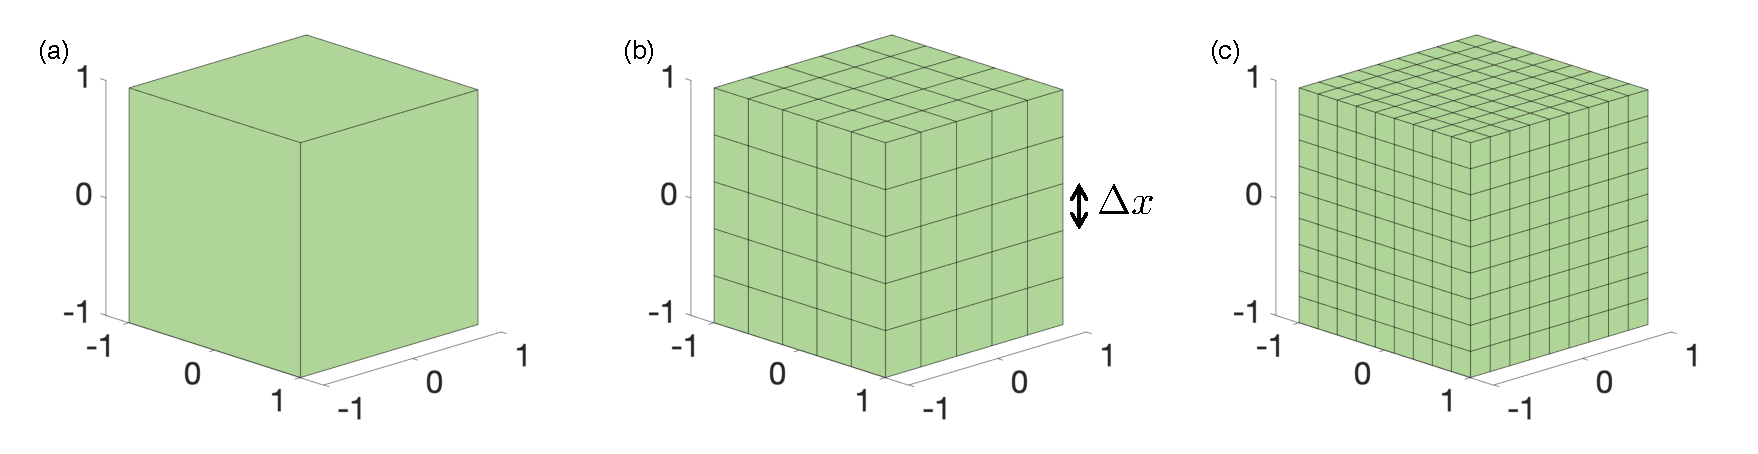
\includegraphics[scale=0.45]{./figures/fig_cube_all_dx}
	\caption{Cubes of various resolutions used for validation. All three cubes have the same volume and contain (a) one interior cube with length $\Delta x = 2$, (b) $5^3 = 125$ interior cubes with length $\Delta x = 2/5$, and (c) $9^3 = 729$ interior cubes with length $ \Delta x = 2/9$. }
	\label{fig_cube_all}
\end{center}
\end{figure}

\subsection{BIE formulations comparison}
{\color{blue} Need to review/edit for writings}\\
In this section, we validate our implementation of both the single- and double-layer methods. We compare both methods since it has been found that the linear system with the single-layer potential formula has larger condition numbers when we integrate its Green's function (Stokeslet) on the aggregate surface, although the single-layer potential has simpler form to use. 
\\
{\color{red}Where is the condition number plot? and cite the papers about this argument}
\\
We compute the total force, $ \vec{F'}_o$, by imposing $\vec{U'}_a = (0,0,-1)$ and $\vec{\Omega'} = (0,0,0)$ in equation (\ref{eq_solid_vel}). To obtain drag ($D'$), we take the settling direction or $z'-$ component of the $ \vec{F'}_o$ on the cube, i.e., 
\begin{align}
	D' = - \vec{F'}_o\cdot \frac{\vec{U'}_a}{\| \vec{U'}_a\|},
\end{align}
where $\| \cdot \|$ is $L^2$ norm.
For both integral methods, the drag values converge to about 25.401. We take this value as our reference drag for error analysis, i.e., $D'_{ex} = 25.401.$
We first compare the drag obtained with varying $\Delta x$ to the previous results in literature in Figure \ref{fig_drag_compare} (a).
\begin{figure}[ht]
	\begin{center}
		\vspace{0.2cm}
		
		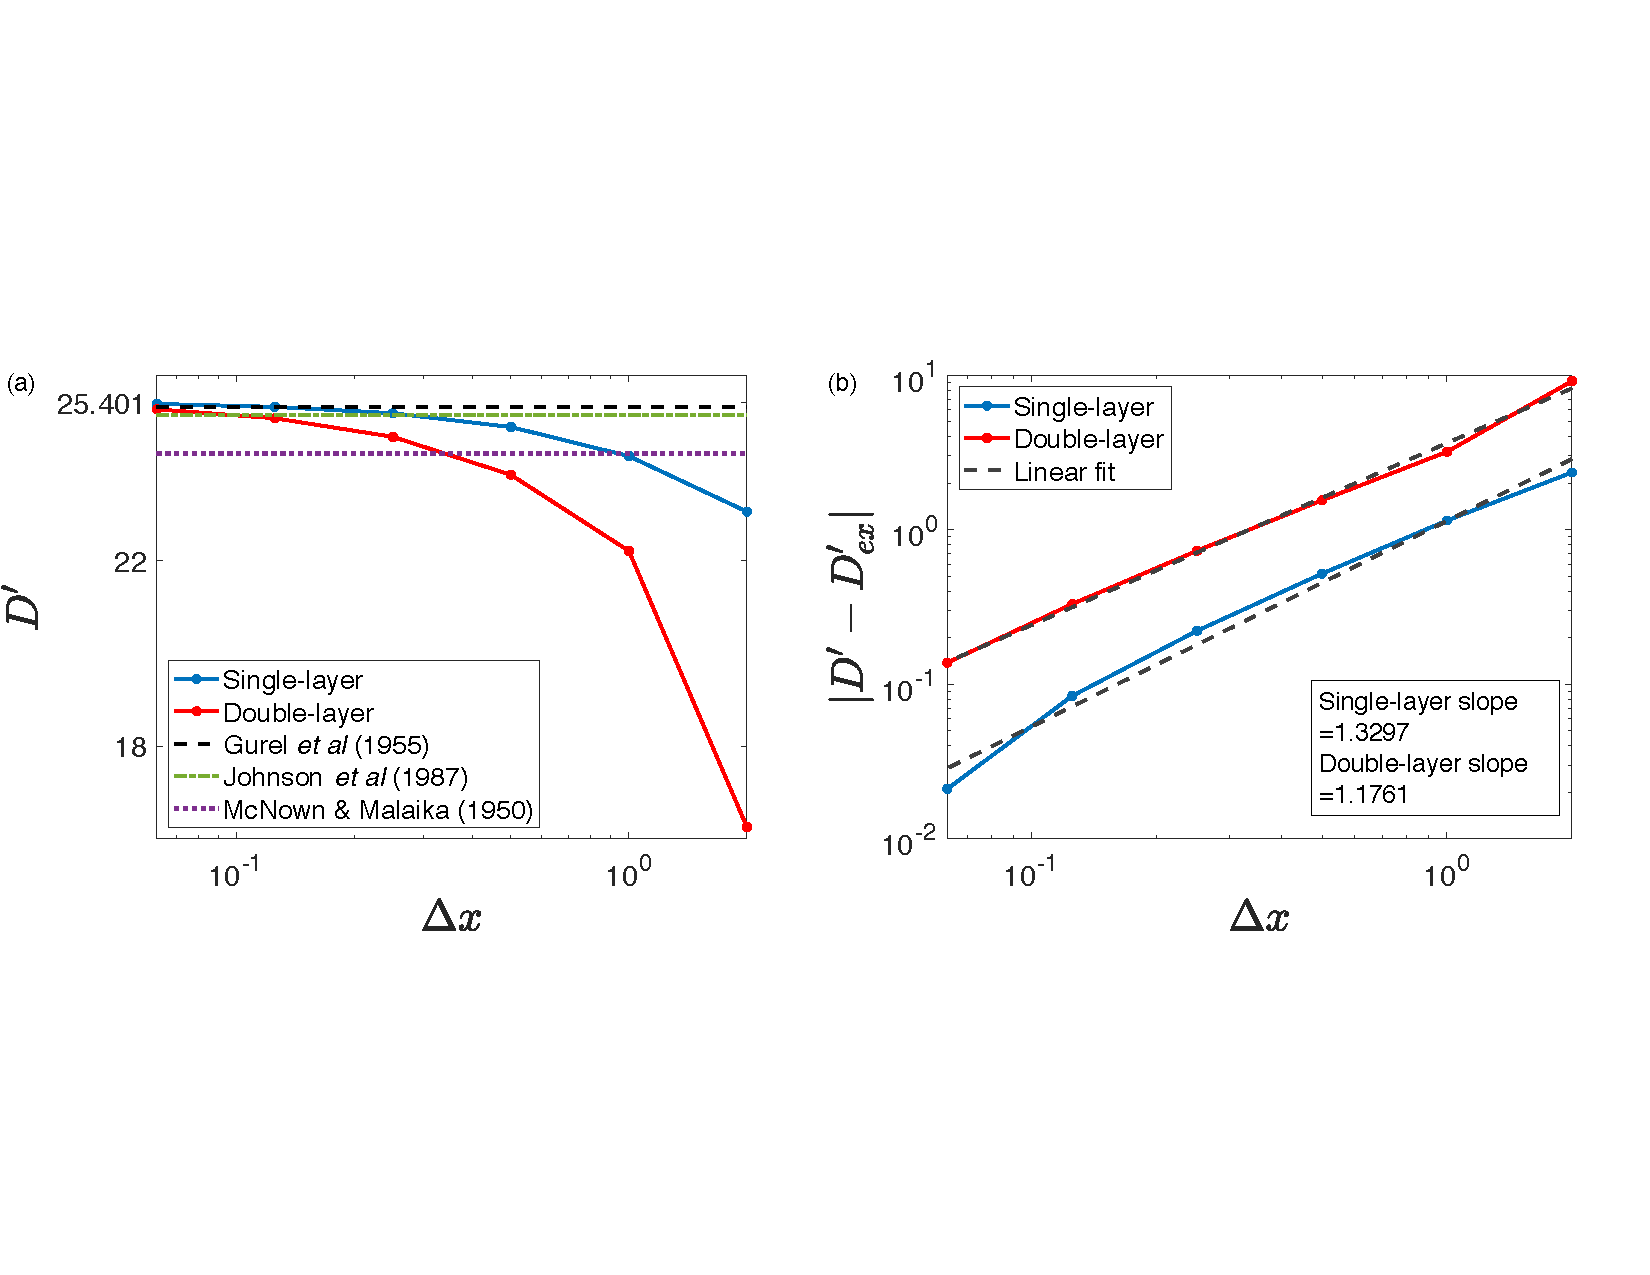
\includegraphics[scale=0.45]{figures/fig_compare_drag_error}
		\vspace{0.2cm}
	
	\caption{(a) Drag on a cube as $\Delta x$ is varied using both the single- and double-layer methods. (b) The error in the drag as $\Delta x$ is varied. A line is fit to the data (dashed line). The error is computed by taking the difference between the limit shown in (a), $25.401$, and drag values when $\Delta x = 2, 1, 0.5,   0.25,  0.125,$ and $0.0625$.}
	\label{fig_drag_compare}
\end{center}
\end{figure}
Our drag, $D'_{ex}$ is comparable with the one found by Gurel {\it{et al.}} \cite{gurel_studies_1955} which is $25.311$ and the empirical relation proposed by Johnson {\it{el al.}}  \cite{johnson_drag_1987} that shows a drag of $25.150$. Earlier McNown \& Malaika \cite{mcnown_effects_1950} presented similar but a somewhat smaller value of $24.311$. 
This implies that our numerical implementation is reliable. In Figure \ref{fig_drag_compare} (b),
we observe the convergence rate that is typically expected to be of a quadratic order when we use the mid-point integration rule in equation (\ref{eq_discretized}). However, we see a convergence rate that is slightly higher than one for both methods. This may come from the presence of edges and corners of cubes. We also notice that the single-layer method shows better accuracy overall.
%
%
\begin{figure}[ht]
	\begin{center}
		\vspace{0.00cm}
		\epsfig{figure=figures/fig_sample_cube_new, scale=0.11}
		
		\vspace{0.25cm}
	\end{center}
	\caption{The shaded face is the domain where the stress vector and density shown in Figs. \ref{fig_stress_cube8_32} and \ref{fig_density_cube8_32} are computed. The red arrow shows the x-axis used in Fig. \ref{fig_cross_section}. Sample streamlines, discussed in next section, are shown as dashed lines.}
	\label{fig_sample_cube}
\end{figure}
\par
Next, we examine whether a vector $\vec{f'}$ or $\vec{\psi'}$ in the $z'-$ direction is constant on the face shown at $z'=1$ as we assume it is for numerical discretization, see Figure \ref{fig_sample_cube}.
 % The shaded square on the top of the cube in Figure \ref{fig_sample_cube} is the face at $z'=1$. 
The single-layer potential formula, in Figure \ref{fig_stress_cube8_32}, shows more constant stress on the square than the double-layer potential, in Figure \ref{fig_density_cube8_32}, as we increase the resolution, although both figures give errors at the corners. This implies that single-layer method allows us to get more accurate results.
\begin{figure}[ht]
	\begin{center}
		\vspace{0.25cm}
		
		\epsfig{figure=figures/fig_stress_all, scale=0.5}
		% \\
		\vspace{0.2cm}
		% \epsfig{figure=figures/fig_density_all.pdf, scale=0.4}
	\end{center}
	\caption{Stress in the $z'-$direction, $\vec{f}_z'$, computed using the single-layer potential, shown at $z'=1$, the face normal to the translational velocity. The resolution is: a) $\Delta x = 2$, b) $\Delta x = 0.5$, and c) $\Delta x =  0.0625$.}
	\label{fig_stress_cube8_32}
\end{figure}
\begin{figure}[h]
	\begin{center}
		\epsfig{figure=figures/fig_density_all.pdf, scale=0.5}
	\end{center}
	\caption{Density in the $z$-direction, $\vec{\psi}_z$,  calculated using the double-layer potential, shown at $z=1$, a face normal to the translational velocity. The resolution is: a) $\Delta x = 2$, b) $\Delta x = 0.5$, and c) $\Delta x =  0.0625$.}
	\label{fig_density_cube8_32}
\end{figure}
%
\\
\par
Moreover, the single-layer potential has a more smooth velocity on a face, as shown in Figure \ref{fig_cross_section}. As we mentioned, the single-layer potential is continuous regardless of the location of points. However, there is a jump on the surface boundary in the double-layer potential formula. When we implement the method, we have to determine if the point is on the surface or the outside of the cube boundary. This may cause oscillatory behavior and has a less smooth transition.
\begin{figure}[ht]
	\begin{center}
		
		\epsfig{figure=figures/fig_vel1d_all.pdf,scale=0.4}
		
		\vspace{0.1cm}
	\end{center}
	\caption{The $z$-component of the velocity along the line $(x,0,1)$ when the cube is placed in a translational flow. The resolution of the cube, $\Delta x$, is varied. Results using the single-layer method (left) and the double-layer method (right) are given. }
	\label{fig_cross_section}
\end{figure}
\\
\par
Based on our investigation on the two boundary integral methods, we concluded that the single-layer method is more accurate and simpler to use for cube-type surfaces.
For this reason, all results in the following sections are obtained using the single-layer formulation. 

\subsection{Validation: Streamlines}
To gain a better understanding of the flow around a cube, we present the streamlines generated when the translational velocity is $\vec{U}'_a = (0,0,-1)$. We show the streamlines around the center of a cube. The sample streamlines locations are shown in Figure \ref{fig_sample_cube} with dashed lines. 
To compute the streamlines, we first obtain the stress vector, $\vec{f}'(\vec{x}'_s)$, on each square face of the cube using equation (\ref{eq_single_nonD}) with our choice of $\vec{U}'_a$.
We then choose initial positions of streamlines below the cube and use a second order Runge-Kutta method to advance the positions in time using the corresponding velocities computed using equation (\ref{eq_single_nonD}. 
We compare the streamlines around four different resolutions of the cube, $\Delta x = 2,1, 0.5,$ and $0.25$. See Figure \ref{fig_streamlines_all}. For the cube with $\Delta x = 2$, streamlines tend to enter the interior of the cube once the lines contact the cube boundary. As we increase the resolution, the streamlines remain exterior to the cube.
Also, higher resolutions result in streamlines following the cube boundary more accurately, showing the convergence of the method.
%
\begin{figure}[ht]
	\begin{center}
		\epsfig{figure=figures/fig_strlns_horizontal-compressed.pdf, width=150mm}
	\end{center}
	\caption{Streamlines around a cube with varying resolution moving in the $z'$-direction. The resolution is: (a) $\Delta x = 2$, (b) $\Delta x = 1$, (c) $\Delta x = 0.5$, and (d) $\Delta x = 0.25$. }
	\label{fig_streamlines_all}
\end{figure}
\subsection{Concentration dynamics}
To quantify the efficiency of transferring organic carbon via settling aggregates, the depth of the fluid or shape of aggregates are typically considered.
In the euphotic zone, which is the uppermost layer of the oceans, the majority of marine aggregates are remineralized by metabolic processes \cite{henson_global_2012}. Omand {\it{et al.}} presented a model to study the sensitivity of the shape of the aggregates with its remineralization rate and density \cite{omand_sinking_2020}. 
Our model of the gravitational sinking aggregates can contribute to understanding the oceanic carbon cycle. We, thus, use the three-dimensional advection-diffusion equation to keep track of concentration dynamics
Note that this model allows us to apply it for any type of concentration, such as salt or temperature. 
In this section, we introduce numerical methods to solve for the concentration, $C$, in time and space and present preliminary results.
\begin{equation}
	\frac{\partial  }{\partial t} C(\vec{x}, t)
	= -\vec{u}(\vec{x}) \cdot \nabla C(\vec{x}, t)
	+ \frac{1}{\text{Pe}} \nabla^2 C(\vec{x}, t),
	\label{eq_ad_diff_3D}
\end{equation}
where $\vec{x} = (x, \ y, z)$ and Pe represents Peclet number describing the ratio between advection and diffusion of the aggregate. 
Note that equation (\ref{eq_ad_diff_3D}) is dimensionless. We non-dimensionalize the time parameter with 
\[
t' = \frac{U_s}{L} t.
\]
Since we apply the moving frame of reference, the fluid velocity, $\vec{u}$, is the sum of the velocity we obtain from the boundary integral method and the settling velocity we prescribed on the aggregate, $\vec{U_a} = (0, \ 0, \ -1)$.
Note that this model allows us to apply it for any type of concentration, such as salt or temperature. 
In this section, we introduce numerical methods to solve for the concentration, $C$, in time and space and present preliminary results.
After careful discussions, we decided to use the second order explicit Runge-Kutta method, due to the efficiency, as follows,
\begin{align}
	k_1 =  f \left( C_j^{n} \right) \Delta t \\ \nonumber
	\\ 
	k_2 = f \left(C_{j+k_1}^{n} \right) \Delta t\\ \nonumber
	\\ 
	C_j^{n+1} = C_j^{n} + \frac{\left(k_1 + k_2 \right)}{2}
\end{align}
An explicit method may cause some stability issues. We therefore need to be careful about and keep tracking the Courant-Friedrichs-Levy (CFL) condition for each advection and diffusion terms,
\begin{equation}
	\max(|u|) \frac{\Delta t}{\Delta x}  \leq 1 \ \ \ \text{for advection, and,}
	\ \  \frac{1}{\text{Pe}}\frac{\Delta t}{\Delta x^2}  \leq 1 \ \ \ \text{for diffusion}.
	\end{equation}
\par
To obtain second order convergence in space with finite differences, we apply  central differences for both the advection and diffusion terms. The first and second derivates of $C$, with respect to $x$, at time level, $n$, can be discretized as
\begin{align}
	\frac{\partial C}{\partial x}  \approx
	 \frac{C_{j+1}^{n} - C_{ j-1}^{n}}{2 \Delta x}
	 \equiv C_1^{FD}
	 \label{eq_c1_fd}
\end{align}
and
\begin{align}
	 \frac{\partial^2 C}{\partial x^2} \approx
	 \frac{C_{ j+1}^n -2 C_{j}^n + C_{ j-1}^n}{\Delta x^2}
	  \equiv C_2^{FD},
	 \label{eq_c2_fd}
\end{align}
respectively. 
Then equation we have
\begin{align}
	 C_{j}^n
	=  -u(x) C_1^{FD} + \frac{1}{\text{Pe}} C_2^{FD}.
\end{align}
\par
One may concern about the stability of the central difference scheme for advection term. However, the oscillation due to the failure of stability condition occurs when we have zero diffusion or sufficiently large Peclet number to be like zero diffusion. As we mentioned, we consider two different sources of diffusion: 1) salinity and 2) heat in temperature $25  ^{\circ}$C.
\par
For salinity of seawater, we find the diffusion coefficient, $D_{salt} = 2 \times 10^{-9}  (\text{m}^2\text{/s})$ from \text{\it Wollast and Garrels (1971)}. In addition, we recall the aggregate's settling speed ($U_s$), its maximum radius ($L$),
\begin{align}
	\text{Pe} 
	= \frac{U_s L }{D_{salt}} 
	\approx \frac{10^{-4}(\text{m/s}) \times \left(5 \times 10^{-4} \right) (\text{m})}{2 \times 10^{-9} (\text{m}^2\text{/s})} = 25
\end{align}
\par 
For the thermal diffusivity, $D_{heat}$, we cosider the value referred by {\it Nayar et. al (2016)} and {\it Sharqawy et. al (2010)},
\begin{align}
	\text{Pe} 
	= \frac{U_s L }{D_{heat}} 
	\approx \frac{10^{-4}(\text{m/s}) \times \left(5 \times 10^{-4} \right) (\text{m})}{1.5 \times 10^{-7} (\text{m}^2\text{/s})} = \frac{1}{3}
\end{align}
(We can also find the pdf file of the seawater properties on \href{http://web.mit.edu/seawater/}{{\color{blue}Thermophysical properties of seawater}.})
Note that this could differ by the size of the aggregate we simulate. This is close to the maximum Peclet number we may expect and may have large diffusion that is enough to use central difference scheme for advection term as well. 
%---------Some results----------------------------------
\section{Results}
$\ \ \ \ \ $  
In order to study the dynamics of marine aggregates in the fluid, we are interested in measuring the forces acting on the aggregates as a response to a background flow. We consider the fluid  flow that is derived from the Taylor expansion of a velocity \cite{guazzelli_physical_2011},
\[
 \vec{U'}_{bg}(\vec{x})
  =  \vec{U'}_{bg}(\vec{x}_0) + 
  \nabla  \vec{U'}_{bg}(\vec{x}_0) \cdot (\vec{x} - \vec{x}_0) + \cdots,
\]
 disturbance up to first-order in space which includes translation, rotation, and extensional flows,
\begin{equation}
 \vec{U'}_{bg}(\vec{x}) = -\vec{U'}_a -  \vec{\Omega'} \times \vec{x'}+\Bar{\Bar{M'}} \cdot \vec{x'},
 \label{eq_bg_flow}
\end{equation}
where $-\vec{U'}_a$ and $\vec{\Omega'}$ are the translational and angular velocities, respectively. 
Moreover, $\bar{\bar{M'}}$ represents a traceless, symmetric second-order tensor that induces extensional or stretching flow. In particular, we consider $\bar{\bar{M'}}$ as compressing in the horizontal direction and stretching in the vertical direction at the same time. 
Note that the background flow, $\vec{U'}_{bg}$, is equivalent to the aggregate's velocity on the surface we prescribed when changing the frame of reference.
We observe each background flow individually in the absence of the other two flows. For example, when we set $\vec{\Omega'} \times \vec{x'} = \vec{0}$ and $\bar{\bar{M'}} \cdot \vec{x'} = \vec{0}$, we observe the force only in the direction of translational flow. 




\subsection{Drag, Torque, and Straining forces}
$\ \ \ \ \ $  
There are three types of forces are induced by each background flow (\ref{eq_bg_flow}):
 1) drag, 2) torque, and 3) straining forces. We analyze these forces acting on aggregates that show better relation with either length scale, $R_g$, defined in equation (\ref{eq_Rg}), or $R_m$, from equation (\ref{eq_Rm}). 
\\
We compute the drag as,
\begin{equation}
\text{D}' =  \Biggl( \int_S' \vec{f'} (\vec{x'}) \ \text{d} S'(\vec{x'}) \Biggr) \cdot \hat{k},
\end{equation}
when setting $\vec{\Omega'}$ and $\bar{\bar{M'}}$ to zero, 
where $\vec{f'}$ is the stress on aggregate surface. 
We expect to see a linear relationship between the drag and a well-chosen length scale, i.e., D$' \sim R$. 
 We present the resulting drag with respect to the gyration radius since we found a clear linear relationship between the two for both IAA and CCA aggregates in Figure \ref{fig_drag}. 
 \begin{figure}[h]
 \begin{center}
    \epsfig{figure=./figures/fig_drag_all_rescaledprime, scale=1}
 \end{center}
 \caption{Drag versus gyration radius. (Left) IAA and (right) CCA aggregates.}
 \label{fig_drag}
 \end{figure}
\par
To observe the torque (T$'$) in the direction of the angular velocity of the aggregate, we now let $\vec{U}'_a$ and $\bar{\bar{M'}}\cdot \vec{x}$ be zero. 
We then calculate the torque as,
\begin{equation}
\text{T}' = 
\int_S' \left( \vec{x'} - \vec{x'}_{cm}  \right) \times \vec{f}(\vec{x'}) \ \text{d}S' (\vec{x'})
 \cdot \frac{\vec{\Omega'}}{\|\vec{\Omega'}\|}.
 \end{equation}
\newline
From the non-dimensional analysis, we expect to see a cubic relationship between torque and a length scale, i.e., $T' \sim R^3$. Figure \ref{fig_torque} shows that both IAA and CCA methods capture the cubic relation with the gyration radius better. We also recognize that IAA shows a more clear relationship than the CCA, since it forms larger aggregates. 
 \begin{figure}[h]
 \begin{center}
    \epsfig{figure=./figures/fig_torque_all, scale=1.05}
 \end{center}
 \caption{Torque versus gyration radius. (Left) IAA and (right) CCA aggregates.}
 \label{fig_torque}
 \end{figure}
\par
We now compute the straining force ($S_f'$) as the response of an aggregate to an extensional flow,
\begin{equation}
S_f' = \vec{E'} \cdot \hat{k}
\end{equation}
where
\begin{equation}
\vec{E'} = \frac{1}{2} \left( 
\int_{S'} \left|\vec{f'} \cdot \hat{v}_i \right| \ \text{d}S'-
\left| \int_S' \vec{f'} \ \text{d} S' \right|\cdot \hat{v}_i
 \right)  \hat{v}_i
 \cdot \frac{\vec{\Omega'}}{\|\vec{\Omega'}\|}.
\end{equation}
Here,  $\vec{f'}$ is the projection of the stress vector in the direction of the eigenvector $\hat{v}_i$.
This eigenvector can be found while we non-dimensionalize this force using the largest eigenvalue in magnitude of $\bar{ \bar{M} }$.
We can decompose the straining force vector as $\vec{E'} = \sum_{i=1}^3 E'_i \hat{v_i}$. 
For the straining force, we expect to observe a quadratic dependence on the aggregate's size. In contrast to the drag and torque, we found a better fit, i.e., $S'_f \sim R^2$ using the maximum radius ($R_m$) as seen in Figure \ref{fig_straining}. 
\begin{figure}[h]
\begin{center}
   \epsfig{figure=./figures/fig_strain_allprime, scale =1}
\end{center}
\caption{Straining forces versus maximum radius. (Left) IAA and (right) CCA aggregates.}
\label{fig_straining}
\end{figure}
\\
\\
This methodology and analysis of forces on settling aggregates has been published in Physical Review Fluids \cite{yoo_hydrodynamic_2020}.
I mainly contributed to comparing the boundary integral equations and implementing the methods to validate, including the streamline simulations. 
%=============concentration simulations================
\subsection{Concentration simulations}
Initially, we set the concentration to zero throughout the fluid domain and higher concentration inside and on the aggregate. For this sample test, an aggregate model made with 10 cubes is used. We first prescribe values of $1$ for the inside of each cube and $0.5$ for all square faces. Also, we put $0.25$ and $0.125$ for all edges and corners of cubes, respectively. This is an intuitive setup for the initial condition to get preliminary results of the advection-diffusion code. However, this might cause a stability problem due to the discontinuity at the aggregate boundaries. Thus, we also simulate with continuous initial concentration using a Gaussian function that has a peak at the center of mass of an aggregate. We adjust the pre-factor of the Gaussian function to have a similar concentration around the aggregate to the discontinuous case. 

Besides the initial concentration, the following conditions are set:
\begin{framed}
\begin{itemize}
	\item Number of cubes (NC) = 10
	%\item $s = 2$; (used to determine the size of domain)
	\item Settling velocity ($\vec{U}_a$) = $(0,0,-1)$
	\item Center of mass of the aggregate ($\vec{x}_{cm}$) = $(-0.8, \  0.4, \ 0)$
	\item Maximum radius of the aggregate ($R_m$) $\approx 5.3472$
	\item Domain = $[-11.50, 9.90] \times [-10.29, 11.09] \times [-21.39, 21.39]$\\
	(Centered at the center of mass of the aggregate.)
	\item Spatial step size: $Nx = Ny = 50, Nz = 100$; $\Delta x = \Delta y = \Delta z \approx 0.43$
	\item Peclet number = 100
	\item Time step (final time = 50): $Nt = 500$; $\Delta t = 0.1$
\end{itemize}
\end{framed}
Note that the settling velocity of an aggregate in a fluid at rest is equivalent to the opposite sign of the translation velocity of the flow past an aggregate, i.e.,  $\vec{U}_a = -\vec{U_s}.$
% For the Peclet number, we consider the aggregate's settling speed ($U_s$), its maximum size ($L$), and the diffusivity ($D$) between $\text{CO}_2$ and water in temperature $25  ^{\circ}$C,
% \begin{align}
% 	\text{Pe}
% 	= \frac{U_s L }{D}
% 	\approx \frac{10^{-4}(\text{m/s}) \times \left(5 \times 10^{-4} \right) (\text{m})}{2 \times 10^{-9} (\text{m}^2\text{/s})} = 25
% \end{align}
% This can differ by the size of the aggregate we consider. This is close to the maximum Peclet number we may expect.However, 
For the Peclet number we set for the sample simulation, in case it is necessary to observe a larger Peclet number which could have more numerical error, we set Pe $=100$ for the initial test case here.
We compute the fluid velocity field once using the boundary integral method and keep it fixed while we update the concentration. 
\par
We simulated this problem using both the implicit (trapezoid), and the explicit (RK2) time integration. Under the conditions provided above, we get an advection CFL condition number of approximately 0.03 and a diffusion one as 0.08. Since the CFL numbers are less than 1, we can use the RK2 method with no stability issue. 
The main reason we wanted to try the explicit method is to reduce computing time if possible. However, we found that both time integration methods gave us similar results in terms of computing time. Before we officially decide which method we are going to use for further research, we will check the order convergence.
\par
We present the snapshots of simulations using the discontinuous and continuous initial concentration in Figure \ref{fig_ic4_trap_snap} and \ref{fig_icG_trap_snap}, respectively. It is a three-dimensional simulation, however, for clear visualization, we slice the domain at $x= -0.8$ which is the middle of $x-$axis.
% We can observe more clearly the aggregate shape in Figure \ref{fig_ic4_trap_snap} due to the discontinuity of the initial concentration.
On the other hand, we see smoother concentration around the aggregate in Figure \ref{fig_icG_trap_snap}. Note that we are using a moving frame of reference such that the surrounding fluid is flowing upward to represent the settling aggregate motion. Assuming $C$ is the concentration of CO$_2$, we can interpret this simulation as dissolving the CO$_2$ gas from the aggregate to the fluid column. 
%r
After time $t \approx 30$ in Figure \ref{fig_icG_trap_snap}, we can see lower concentration is going outside of our numerical domain.  
 \begin{figure}[h]
 \begin{center}
	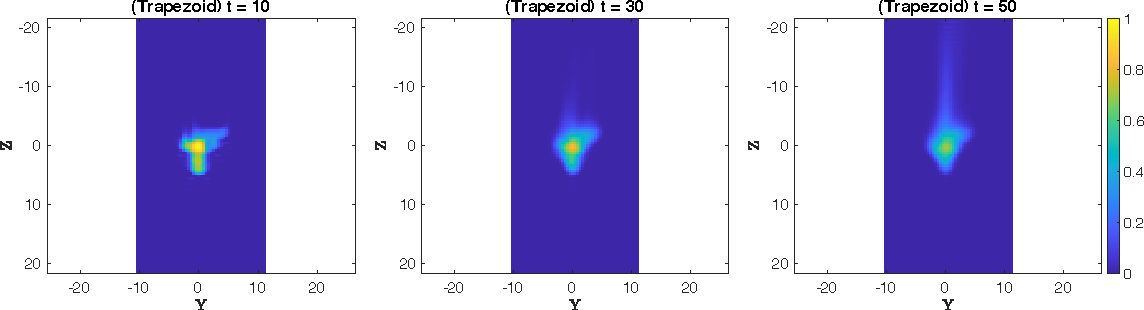
\includegraphics[scale=0.7]{./figures/fig_ic4_Trap_snap135}
 \end{center}
 \caption{Discontinuous initial concentration with finite differences space and trapezoid time method.}
 \label{fig_ic4_trap_snap}
 \end{figure}
 %
 % icG trap
 %
 \begin{figure}[h]
 \begin{center}
	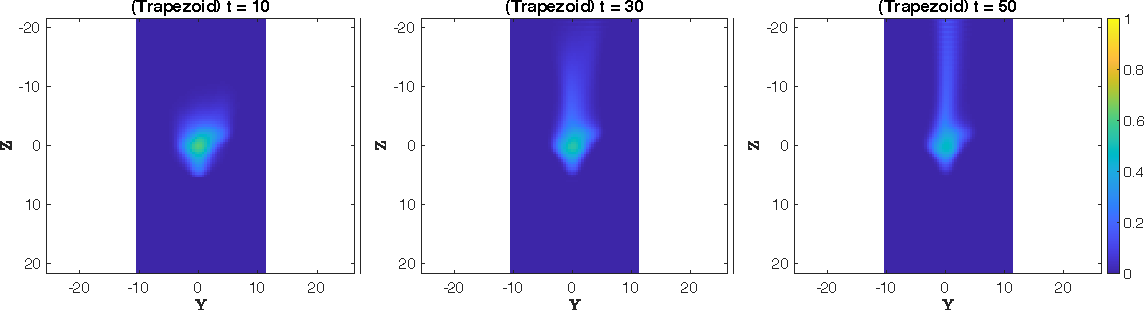
\includegraphics[scale=0.7]{./figures/fig_icG_Trap_snap135}
 \end{center}
 \caption{Continuous initial concentration with finite differences space and trapezoid time method.}
 \label{fig_icG_trap_snap}
 \end{figure}
\par
Figure \ref{fig_sumC} shows that the sum of the concentration of the fluid over time. We see that the total concentration begins to decay approximately after $t \approx 20$ with continuous initial condition (orange line).
The results seems to be consistent with our expectation that the mass is conserved until the flow reaches the upper boundary of our domain. The right plot in Figure \ref{fig_sumC} shows the error between the total concentration at each time and initial one up to time $t = 20$. We see that the error increases over the time for both initial condition cases.  
 \begin{figure}[ht]
 \begin{center}
    \epsfig{figure=./figures/fig_sumC_test.eps, scale = 0.3}
	%  \hspace{5mm}
	\epsfig{figure=./figures/fig_sumC_error.eps, scale = 0.3}
 \end{center}
 \caption{(Left) Variation of total concentration in fluid domain in time. (Right) Error between the total concentration at each time and initial sum of concentration.}
 \label{fig_sumC}
 \end{figure}

